\documentclass[12pt]{article}
\usepackage[margin=1in]{geometry} 
\usepackage{natbib}
\usepackage{graphicx}
\usepackage{amsmath}
\usepackage{tikz}
\usetikzlibrary{backgrounds}

\title{Thaumaturgical Cosmology and Metaphysics of the Soluna-Gaia Universe}
\author{Dr. Claude Hermes}
\date{March 2024}

\begin{document}

\maketitle

\begin{abstract}
This paper presents a comprehensive overview of the cosmological structure and metaphysical principles underlying magic in the Soluna-Gaia universe (SGU). Through analysis of thaumaturgical phenomena and historical records, we posit a model for the fundamental forces and entities that shape the SGU. Central to this cosmology are the celestial bodies of Sun, Moon, and Earth, which serve as both physical and magical anchors for the universe. The interactions and balance between these primal forces give rise to the laws of magic and the potential for mortal practitioners to shape reality. We explore the mechanisms of spellcasting, the nature of magical energy, and the implications of celestial dynamics on thaumaturgical practice. Additionally, we examine key historical events such as the Convergence and the Fracturing to contextualize the development of magical theory and society in the SGU. 
\end{abstract}

\section{1. Introduction}
The Soluna-Gaia universe (SGU) is a realm in which magic is an inextricable component of the physical and metaphysical structure of reality. Thaumaturgy in the SGU is not merely the province of esoteric mysticism or superstition, but a natural force woven into the fabric of existence, which can be studied, understood, and harnessed. The systematic study and practice of magic has shaped the development of SGU civilizations and given rise to complex magical traditions, academies, and sociopolitical structures.

At the heart of SGU magic lie the three Prime Elements: Sun, Moon, and Earth. These celestial bodies are more than simple astronomical objects; they are the physical manifestations of the universe's fundamental metaphysical principles. The Sun represents the raw, unfiltered energy of creation and destruction, the Moon embodies change, transformation, and the mutable nature of reality, while the Earth signifies stability, physicality, and the foundation of life \citep{Valdis2017}. The interplay and balance between these primal forces gives rise to the various expressions of magic observed in the SGU.

In this paper, we present a comprehensive model of SGU magical cosmology and metaphysics derived from analysis of both contemporary thaumaturgical research and historical accounts. Section 2 examines the role of the Prime Elements as the basis for magic. Section 3 describes the mechanics of spellcasting and the different magical disciplines. Section 4 explores the metaphysical implications of solar-lunar-terrestrial interactions, including the phenomena of eclipses and celestial convergences. Section 5 situates our magical model in the context of key historical events and thaumaturgical paradigm shifts. Finally, Section 6 offers concluding remarks and directions for future research.

% paste begin
\section{2. The Prime Elements and Magic}

The three Prime Elements - Sun, Moon, and Earth - are the cornerstones of magic in the Soluna-Gaia universe (SGU). These celestial bodies are not merely astronomical objects, but physical anchors for the metaphysical domains that suffuse the SGU with magical energy. Each Prime Element represents a fundamental aspect of reality and gives rise to a distinct form of magic with its own properties, laws, and manifestations.

\begin{figure}[htb]
    \centering
    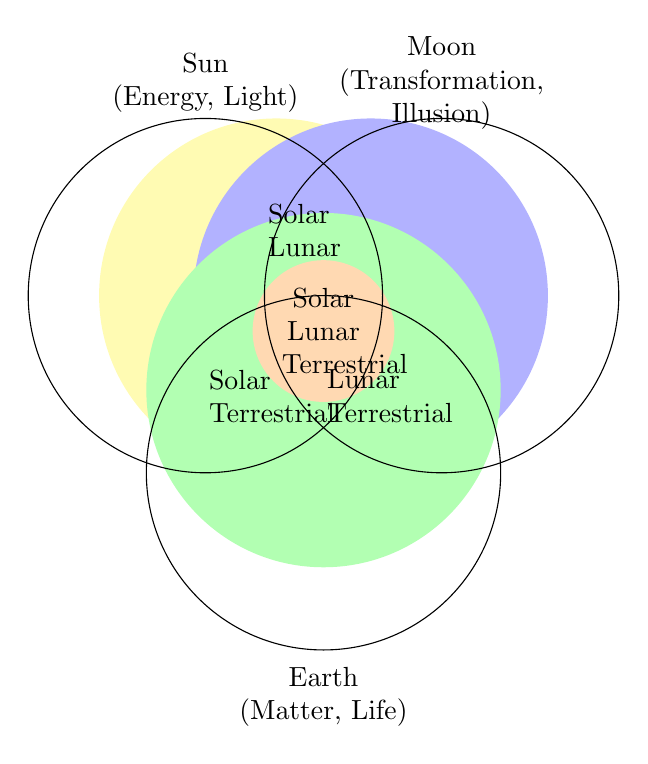
\begin{tikzpicture}[scale=1.5]
        % Draw the circles
        \draw (0,0) circle (1.5cm) node [text=black,align=center] at (0, 1.8) {Sun\\(Energy, Light)};
        \draw (2,0) circle (1.5cm) node [text=black,align=center] at (2, 1.8) {Moon\\(Transformation,\\Illusion)};
        \draw (1,-1.5) circle (1.5cm) node [text=black,align=center] at (1, -3.4) {Earth\\(Matter, Life)};

        % Fill the overlapping regions
        \begin{scope}[on background layer]
            \fill[yellow!30] (0.6,0) circle (1.5cm);
            \fill[blue!30] (1.4,0) circle (1.5cm);
            \fill[green!30] (1,-0.8) circle (1.5cm);
            \fill[orange!30] (1,-0.3) circle (0.6cm);
        \end{scope}
        
        % Add labels for the overlapping regions
        \node[text width=4em] at (1,0.55) {Solar\\Lunar};
        \node[text width=4em] at (0.5,-0.85) {Solar\\Terrestrial};
        \node[text width=4em] at (1.5,-0.85) {Lunar\\Terrestrial};
        \node[text width=3em,align=center] at (1,-0.3) {Solar\\Lunar\\Terrestrial};
    \end{tikzpicture}
    \caption{The overlapping domains and properties of the three Prime Elements: Sun, Moon, and Earth.}
    \label{fig:prime_elements_venn}
\end{figure}

The Sun is the wellspring of raw, primal energy that fuels the fires of creation and destruction. Its magic is characterized by heat, light, and sheer power. Solar mages draw upon this energy to conjure searing flames, project beams of brilliant radiance, and infuse their spells with overwhelming force. The Sun's magic is intense and immediate, but also short-lived; it cannot be stored or channeled for long periods, only unleashed in bursts of potency. Solar magic excels at offensive spellcraft, purification rituals, and workings that require a sudden influx of energy. However, it struggles with subtlety and finesse, and can easily cause collateral damage if not carefully controlled.

In contrast, the Moon represents the ever-shifting face of reality, the interplay of light and shadow, truth and illusion. Lunar magic is fluid, elusive, and ethereal. It deals in deception, transformation, and the manipulation of perceptions. Lunar mages can weave glamours to disguise their appearance, cast phantasms to confuse and mislead, and even reshape their physical form. The Moon's magic is also closely tied to the cycles of life, death, and rebirth; it holds sway over the tides of emotion, the ebb and flow of vitality, and the mysteries of the soul. Lunar magic excels at illusions, shapeshifting, divination, and subtle mental influence. However, its effects are always temporary and subject to the ever-changing whims of the Moon.

The Earth is the foundation upon which all life and matter rest. It represents stability, resilience, and the enduring power of nature. Terrestrial magic is rooted in the physical world and draws strength from the bones of the earth. Terrestrial mages can manipulate stone and soil, commune with plants and animals, and infuse objects with protective enchantments. The Earth's magic is slow and steady, but also incredibly resilient; it can weather any storm and outlast any foe. Terrestrial magic excels at defensive wards, healing spells, and the crafting of magical items and constructs. However, it is limited by its need for a physical medium to work through, and cannot directly affect the mind or soul.

Each type of magic is governed by a complex web of metaphysical laws and principles that define its capabilities and limitations. These laws are not arbitrary rules, but fundamental expressions of the nature of the Prime Elements themselves. For example, the law of conservation of energy dictates that Solar magic cannot create or destroy energy, only convert it from one form to another. The law of entropy ensures that all Lunar transformations must eventually revert to their original state. The law of equivalent exchange requires that Terrestrial magic must always balance the forces of creation and destruction, giving and taking in equal measure.

Mages in the SGU are born with an innate attunement to one of the Prime Elements, which shapes their magical abilities and inclinations. A mage's attunement is believed to be determined by the alignment of the celestial bodies at the moment of their birth, and the balance of elemental energies in their soul. Solar mages tend to be passionate, ambitious, and fearless, but also reckless and quick to anger. Lunar mages are often intuitive, adaptable, and enigmatic, but also capricious and prone to melancholy. Terrestrial mages are usually patient, reliable, and nurturing, but also stubborn and resistant to change.

However, a mage's attunement does not wholly define them or limit their potential. With study and practice, mages can learn to cast spells from any of the three arcane disciplines, blending the unique strengths of each into potent magical effects. The most skilled and versatile mages are those who have mastered the art of weaving together Solar, Lunar, and Terrestrial energies into seamless spells. These rare individuals are known as Triune Adepts, and are revered as the pinnacle of magical achievement in the SGU.

The interplay between the Prime Elements gives rise to a vast array of magical phenomena and practices. Solar and Lunar magic can be combined to create illusions of dazzling beauty and terrifying power, or to shape the very fabric of space and time. Solar and Terrestrial magic can be fused to conjure living flames that grow and spread like wildfire, or to imbue objects with the strength and resilience of the earth. Lunar and Terrestrial magic can be woven together to create shapeshifting chimeras, or to summon forth the spirits of nature.

The balance between the Prime Elements is not static, but rather a dynamic equilibrium that is constantly shifting and evolving. The waxing and waning of the Moon, the turning of the seasons, and the movement of the celestial bodies all influence the flow of magical energy in the SGU. When the Sun and Moon align in a solar eclipse, their opposing energies collide and unleash chaos, twisting magic into unpredictable and dangerous forms. Conversely, when the Sun, Moon, and Earth align in a perfect syzygy, their energies resonate in harmony, amplifying magic to awe-inspiring heights and enabling workings of world-shaping power.

These celestial events have played a pivotal role in the history of the SGU, shaping the rise and fall of civilizations, the birth and death of gods, and the fate of entire planes of existence. The Convergence of the Primal Suns, which occurs once every ten thousand years, is said to have triggered the ascension of the first mortal mages and the dawn of the mythic age. The Fracturing of the Moons, which split the original moon into its current triune form, is believed to have unleashed a cataclysm that shattered continents and birthed new oceans. The Dance of the Earthen Stars, a rare alignment of the planets that takes place once a century, is associated with the emergence of powerful Terrestrial artifacts and the awakening of slumbering ley lines.

The study of astronomy and astrology is thus inextricably linked to the practice of magic in the SGU. Mages seek to understand the intricate relationships between the celestial bodies and the Prime Elements, and to predict the ebb and flow of magical energy that they generate. The movements of the stars and planets are carefully charted and analyzed, their positions and aspects used to divine the optimal times for casting spells and performing rituals. The most skilled astromancers can even attune themselves to the cosmic rhythms of the universe, drawing upon the power of the heavens to fuel their magic and shape their destiny.

However, the connection between magic and the celestial bodies is not a one-way street. Just as the Prime Elements shape the nature of magic, so too does the practice of magic influence the balance of the elements. Every spell cast, every ritual performed, every magical working unleashed sends ripples through the fabric of reality, subtly altering the flow of elemental energy. Over time, these ripples can build into waves, and waves into tides, shifting the balance of power between the Prime Elements and changing the very nature of magic itself.

This is the great responsibility and burden of the mages of the SGU: to use their power wisely and judiciously, to maintain the delicate balance between the elements, and to preserve the stability of the universe itself. Those who abuse their magic, who seek to dominate or destroy, who upset the natural order of things, risk unleashing catastrophe upon the world. The Shattering of the Skies, the Unraveling of the Weave, the Sundering of the Stones - these are the dire consequences of unchecked magical ambition, the result of mages who sought to wield power beyond their understanding or control.

And yet, despite the dangers, the allure of magic endures. For those with the talent and the will, the ability to shape reality itself is a siren song that cannot be ignored. The path of the mage is one of endless discovery and infinite potential, a journey that leads to the very heights of power and the very depths of understanding. To walk this path is to embrace both the wonders and the perils of magic, to accept the responsibility of stewardship over the forces that shape the universe, and to strive for the wisdom and balance needed to wield them safely.

In the end, the true power of magic in the SGU lies not in the flashy spells or the awe-inspiring rituals, but in the understanding and mastery of the fundamental forces that underlie all of reality. The Prime Elements are the building blocks of the universe, the raw materials from which all things are made. To know them, to understand them, to wield them with skill and care - that is the essence of magic, and the ultimate goal of every mage in the Soluna-Gaia universe.

So let us delve deeper into the mysteries of the Sun, the Moon, and the Earth, and explore the myriad ways in which their magic weaves through the tapestry of the SGU. Let us study the laws and principles that govern the Prime Elements, and learn to harness their power for the betterment of all. And let us never forget the great responsibility that comes with the gift of magic, the duty to use it wisely and well, to preserve the balance and harmony of the universe, and to pass on our knowledge to the generations to come.

For in the end, the magic of the Soluna-Gaia universe is not just a tool or a weapon, but a sacred trust, a divine spark that burns within the heart of every mage. To wield it is to touch the very fabric of creation, to shape the destiny of worlds, and to leave an indelible mark upon the great canvas of existence. May we all prove worthy of this trust, and may the light of magic guide us ever onward, to the stars and beyond.
% paste end 
% \begin{itemize}
%     \item \textbf{Solar Magic:} Solar magic is characterized by raw power, heat, and radiance. Its spells focus on conjuring and projecting energy in various forms, such as solar flares, beams of searing light, and auras of vitalizing warmth. Solar magic excels at enhancing the potency of other spells. Healing magic fueled by Solar energy tends to focus on purging disease and restoring vigor. Solar mages often have a natural affinity for pyromancy and photomancy as well. 
%     
%     \item \textbf{Lunar Magic:} Lunar magic is characterized by mutability, illusion, and subtle influence. Its spells revolve around shapeshifting, sensory deception, divination, and mental manipulation. Lunar magic allows practitioners to blur the lines of reality, crafting glamours and illusions that fool the eye and mind. It is also tied to the cycles of life, death, and rebirth. Healing magic drawing on Lunar energy specializes in regeneration and purging toxins.
%     
%     \item \textbf{Terrestrial Magic:} Terrestrial magic is characterized by stability, physicality, and vitality. Its spells focus on manipulating earthen matter, attuning to the life force of flora and fauna, and reinforcing objects and structures. Terrestrial magic excels at defensive wards and barriers. It is also essential for the crafting of magical items and constructs. Healing magic rooted in Terrestrial energy mends bones and flesh.
% \end{itemize}
% 
% Each type of magic is governed by specific metaphysical principles and laws that constrain the scope and potency of spellcasting \citep{Lumina2009}. For example, Lunar magic cannot create permanent changes; any transformations it enacts will always revert in time. Solar magic dissipates quickly and cannot be stored, only channeled or expended. Terrestrial magic requires a physical medium to work through and cannot directly affect the mind or soul.
% 
% Mages in the SGU are typically attuned to one Prime Element, which determines their magical aptitudes and specialties. However, most can learn to cast spells across all three disciplines to varying degrees. Only the most gifted and dedicated practitioners can master the art of combining multiple types of magic into a single spell. The Empyreal Adepts of the Second Era were said to work miracles that merged Solar radiance, Lunar cunning, and Terrestrial might \citep{Faelyn2012}.
% 
% The strength of magic in the SGU waxes and wanes in cycles tied to the movement of the celestial bodies. During a solar eclipse, magic becomes twisted and erratic, prone to eldritch side-effects. Conversely, during a syzygy, when the Sun and Moon align with the Earth, magic swells to new heights, allowing for workings of extraordinary power. These celestial events, and the concomitant surges in magical energy, have often been pivotal moments in the history of the SGU \citep{Arathar2018}.
% 
% \begin{figure}[h]
%     \centering
%     \includegraphics[width=0.8\textwidth]{PrimeElements.png}
%     \caption{The three Prime Elements and their associated magical properties.}
%     \label{fig:PrimeElements}
% \end{figure}

% Additional sections (3-5) would follow, further elaborating on spellcasting mechanics, celestial metaphysics, and historical context.
% section3 paste begin
\section{3. Spellcasting Mechanics and Arcane Disciplines}

The art of spellcasting in the Soluna-Gaia universe is a complex and multifaceted discipline, requiring a deep understanding of the metaphysical principles that govern the Prime Elements, as well as extensive practice in the techniques of magical manipulation. At its core, spellcasting involves the channeling and shaping of elemental energies into specific patterns and forms, which then manifest as tangible effects upon the world.

\begin{figure}[htb]
    \centering
    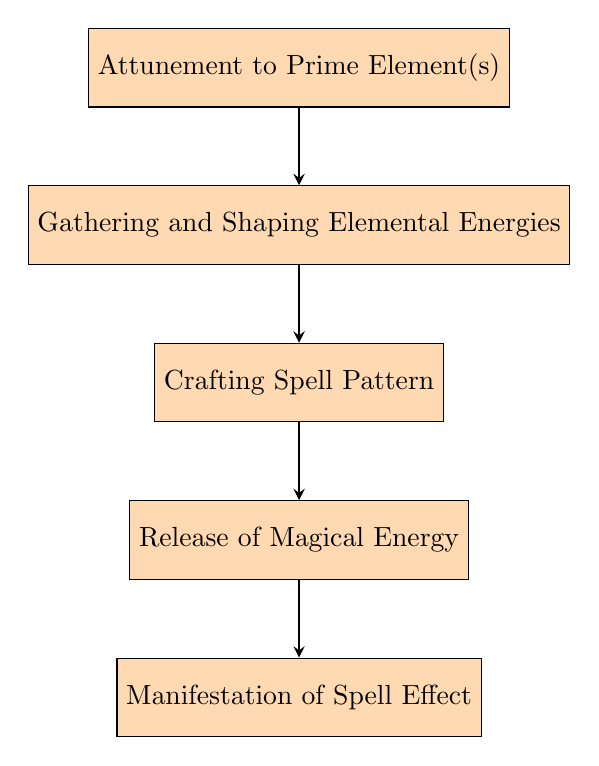
\begin{tikzpicture}[node distance=2cm]
        \tikzstyle{process} = [rectangle, minimum width=3cm, minimum height=1cm, text centered, draw=black, fill=orange!30]
        \tikzstyle{arrow} = [thick,->,>=stealth]
        
        \node (attunement) [process] {Attunement to Prime Element(s)};
        \node (gathering) [process, below of=attunement] {Gathering and Shaping Elemental Energies};
        \node (crafting) [process, below of=gathering] {Crafting Spell Pattern};
        \node (release) [process, below of=crafting] {Release of Magical Energy};
        \node (manifestation) [process, below of=release] {Manifestation of Spell Effect};
        
        \draw [arrow] (attunement) -- (gathering);
        \draw [arrow] (gathering) -- (crafting);
        \draw [arrow] (crafting) -- (release);
        \draw [arrow] (release) -- (manifestation);
    \end{tikzpicture}
    \caption{The process of spellcasting, from attunement to manifestation.}
    \label{fig:spellcasting_flowchart}
\end{figure}

The process of casting a spell begins with the mage drawing upon their innate connection to one or more of the Prime Elements, attuning themselves to the flow of magical energy that suffuses the universe. This attunement can be achieved through various means, such as meditation, ritual invocations, or the use of enchanted foci and reagents. Each mage has their own unique methods and preferences for tapping into the wellsprings of magic, honed through years of study and experimentation.

Once attuned, the mage must then gather and shape the raw elemental energies into a coherent spell pattern. This is where the true skill and artistry of spellcasting comes into play, as the mage must weave the disparate strands of magic into a harmonious whole, balancing the forces of creation and destruction, light and shadow, stability and change. The spell pattern is essentially a blueprint or schematic for the desired effect, a precise arrangement of magical energies that, when released, will alter reality in accordance with the mage's will.

Crafting a spell pattern is a delicate and intricate process, requiring intense concentration, visualization, and a deep intuitive understanding of the interplay between the elements. Mages must be able to sense the ebb and flow of magical currents, to anticipate how different energies will interact and combine, and to make split-second adjustments to maintain the stability and integrity of the spell. Even the slightest miscalculation or imbalance can cause the spell to unravel or backfire, often with disastrous consequences.

The complexity and power of a spell are determined by several factors, including the number and type of Prime Elements involved, the intricacy of the spell pattern, and the skill and experience of the caster. A simple cantrip to light a candle might require only a minor twist of Solar energy, while a world-shaking ritual to rend the fabric of reality could involve all three elements woven into a mind-bendingly complex matrix. Generally speaking, the more elements involved and the more sophisticated the pattern, the more challenging and taxing the spell will be to cast.

Once the spell pattern is complete, the mage must then release the pent-up magical energies, channeling them through their body and will to manifest the desired effect. This release can take many forms, from a whispered incantation to a dramatic gesture to a burst of raw elemental power. The method of release often varies based on the nature of the spell and the personal style of the caster, but all require a final act of will and focus to unleash the magic upon the world.

The manifestation of a spell can be instantaneous or gradual, subtle or spectacular, depending on its nature and intent. A bolt of searing Solar fire might erupt from the mage's hand and streak towards its target, while a Lunar glamour might slowly shimmer into existence, cloaking the caster in an illusory disguise. A Terrestrial healing spell might knit bones and flesh back together with gentle warmth, while a combined elemental blast might rend the earth, boil the seas, and set the very air ablaze.

Regardless of its form or effect, every spell leaves an indelible mark upon the fabric of reality, a ripple in the cosmic web of magic that can be sensed by those attuned to such things. The more powerful the spell, the more profound and far-reaching its impact will be, both on the immediate environment and on the overall balance of the Prime Elements. A great work of magic can shift the tides of history, reshape the landscape of the world, and even attract the attention of gods and other cosmic entities.

Given the complexity and potential consequences of spellcasting, it is no surprise that the study and practice of magic in the SGU is a highly regulated and structured affair. Mages are typically trained within established arcane disciplines, each with its own unique focus, philosophy, and techniques. These disciplines provide a framework for understanding and manipulating the Prime Elements, as well as a set of ethical guidelines and practical safeguards to ensure the responsible use of magic.

The three main arcane disciplines in the SGU are Solar, Lunar, and Terrestrial, each corresponding to one of the Prime Elements. Solar mages, also known as Solarians or Helions, specialize in the manipulation of raw energy, light, and heat. They are the masters of offensive magic, able to conjure searing flames, blinding radiance, and devastating blasts of pure power. Solarians are often found in roles that require decisive action and overwhelming force, such as combat mages, demon hunters, and arcane enforcers.

Lunar mages, also known as Lunarians or Selenites, specialize in the manipulation of illusion, transformation, and the subtle arts of the mind. They are the masters of deception and misdirection, able to weave glamours that fool the senses, assume alternate forms, and influence the thoughts and emotions of others. Lunarians are often found in roles that require subtlety and finesse, such as spies, diplomats, and courtiers.

Terrestrial mages, also known as Terrans or Geomancers, specialize in the manipulation of matter, life, and the forces of nature. They are the masters of defensive magic, able to shape stone and metal, commune with plants and animals, and imbue objects with protective enchantments. Terrans are often found in roles that require stability and nurturing, such as healers, crafters, and guardians.

While most mages specialize in one of these three disciplines, it is not uncommon for individuals to study multiple paths, blending the techniques and philosophies of different elements into a unique and versatile style of magic. These multi-disciplinary mages, known as Arcanists or Mystics, are highly prized for their adaptability and broad range of skills, and often serve as advisors, researchers, or explorers.

Beyond the three main disciplines, there are also a number of more specialized or esoteric schools of magic, each with its own unique focus and techniques. These include Chronomancy (the manipulation of time), Necromancy (the manipulation of death and undeath), Divination (the art of seeing the future and the hidden), and many others. These schools are often seen as more advanced or dangerous than the mainstream disciplines, and are typically only studied by the most experienced and daring of mages.

Regardless of their chosen discipline or specialization, all mages in the SGU are expected to adhere to a strict code of ethics and responsibility in the use of their powers. The abuse or misuse of magic is considered a grave offense, and can result in severe penalties, including the stripping of magical abilities, exile from arcane society, or even execution in extreme cases. Mages are taught from an early age to respect the power they wield, to use it only for the greater good, and to always consider the consequences of their actions.

This sense of responsibility is reinforced by the various magical organizations and institutions that exist throughout the SGU, from the great arcane academies and libraries to the local covens and guilds. These groups provide a support network for mages, offering training, resources, and a sense of community, but also serve as watchdogs and regulators, ensuring that the use of magic remains within acceptable bounds.

One of the most important of these organizations is the Arcanum, a pan-dimensional order of mages dedicated to the study and preservation of magical knowledge, as well as the maintenance of balance and stability across the multiverse. The Arcanum is composed of some of the most powerful and wise mages from all disciplines and walks of life, and serves as a neutral arbiter and peacekeeper in magical affairs. Its members are sworn to uphold the highest ideals of magic, and to intervene in any situation that threatens the integrity of the cosmic order.

Despite the best efforts of the Arcanum and other magical institutions, however, the use of magic in the SGU remains a constant source of tension and conflict. There are always those who seek to exploit magic for personal gain or power, who push the boundaries of what is acceptable or safe, or who delve into forbidden and dangerous practices. The battle against magical corruption and abuse is an ongoing one, fought in the halls of power, the shadows of the underworld, and the very fabric of reality itself.

At the same time, magic also represents one of the greatest hopes and aspirations of the beings of the SGU. It is a tool for creation and discovery, a means of transcending the limitations of the physical world and touching the divine. It is a source of wonder and inspiration, a reminder of the infinite potential that lies within every soul. To study magic is to embark on a journey of self-discovery and transformation, to unlock the secrets of the universe and to tap into the very essence of life itself.

In the end, the art of spellcasting in the Soluna-Gaia universe is a reflection of the duality that lies at the heart of magic itself. It is both a great power and a great responsibility, a force for creation and destruction, a path to enlightenment and a road to damnation. It is the fire that burns within the heart of every mage, the spark that ignites the imagination and the will. And it is the key to shaping the destiny of the SGU, for good or for ill, for all eternity.
% section 3 paste end

% section 4 paste begin
\section{4. Celestial Dynamics and the Metaphysics of Magic}

The interplay between the celestial bodies and the Prime Elements is one of the most fundamental and far-reaching aspects of magic in the Soluna-Gaia universe. The Sun, Moon, and Earth are not merely passive sources of magical energy, but active participants in the cosmic dance of creation and destruction, constantly shaping and being shaped by the ebb and flow of elemental forces.

At the heart of this celestial dynamic lies the concept of resonance, the idea that the Prime Elements are attuned to specific frequencies or vibrations that echo throughout the fabric of reality. Each element has its own unique resonance, a cosmic signature that defines its nature and governs its interactions with the other elements and the wider universe.

The Sun, for example, resonates with the frequency of raw, primal energy, the fundamental vibration of creation and destruction that underlies all existence. This solar resonance is what gives Solarian magic its incredible power and intensity, allowing mages to tap into the very essence of the universe and channel it into their spells. However, it is also what makes Solar magic so volatile and dangerous, as the slightest imbalance or disruption in the solar frequency can unleash devastating consequences.

The Moon, on the other hand, resonates with the frequency of change and transformation, the endless cycle of growth and decay, light and shadow. This lunar resonance is what gives Lunarian magic its fluid and mutable nature, allowing mages to manipulate the very essence of reality and shape it to their will. However, it is also what makes Lunar magic so unpredictable and elusive, as the lunar frequency is constantly shifting and adapting, making it difficult to control or contain.

The Earth, finally, resonates with the frequency of stability and permanence, the immutable laws of matter and energy that hold the universe together. This terrestrial resonance is what gives Terran magic its enduring strength and resilience, allowing mages to tap into the fundamental forces of nature and use them to create lasting change in the world. However, it is also what makes Terrestrial magic so slow and inflexible, as the terrestrial frequency is resistant to change and slow to adapt to new circumstances.

These elemental resonances are not static or fixed, but are constantly shifting and evolving in response to the movements and alignments of the celestial bodies. As the Sun, Moon, and Earth orbit and rotate around each other, their relative positions and angles create complex patterns of interference and amplification, which in turn affect the flow and balance of magical energy throughout the universe.

The most dramatic and consequential of these celestial alignments are the eclipses, rare and powerful events that occur when the Sun, Moon, and Earth align in a straight line, casting a shadow across the face of one or more of the celestial bodies. During a solar eclipse, the Moon passes directly between the Sun and the Earth, blocking the solar resonance and plunging the world into darkness. This sudden absence of Solar energy creates a void in the fabric of magic, which is quickly filled by the chaotic and unpredictable energies of the Lunar and Terrestrial elements.

The result is a period of intense magical instability, where the normal laws and principles of magic break down and anything becomes possible. Spells that would normally be impossible or forbidden become suddenly feasible, while even the simplest and most mundane of magics can go wildly awry. Mages who are caught unprepared during a solar eclipse can find themselves overwhelmed by the surge of wild magic, their carefully crafted spells unraveling into chaotic and destructive forces.

During a lunar eclipse, on the other hand, the Earth passes directly between the Sun and the Moon, casting its shadow across the lunar surface. This alignment blocks the Lunar resonance, but also creates a unique configuration where the Solar and Terrestrial energies are focused and amplified through the lens of the Earth. The result is a period of intense magical clarity and power, where spells become more potent and precise, and the boundaries between the physical and the mystical become blurred.

Mages who are attuned to the lunar eclipse can tap into this amplified magical energy to achieve feats that would normally be impossible, such as opening portals to other dimensions, communicating with the spirits of the dead, or even altering the very fabric of reality itself. However, the lunar eclipse is also a time of great danger, as the focused magical energies can easily overwhelm the unprepared or the reckless, leading to madness, possession, or even physical transformation.

Beyond the eclipses, there are countless other celestial alignments and configurations that can affect the flow and balance of magic in the SGU. The phases of the Moon, for example, have a profound impact on the strength and nature of Lunar magic, with spells cast under the full Moon being particularly potent and unpredictable, while those cast under the new Moon are more subtle and introspective. Similarly, the position of the planets and stars can create complex patterns of resonance and interference that can enhance or disrupt specific types of magic, depending on their elemental affinities and symbolic associations.

The study of these celestial dynamics is a central concern of magical theory and practice in the SGU, with entire schools and disciplines devoted to understanding and harnessing the power of the heavens. Astromancers, for example, specialize in using the positions and movements of the celestial bodies to predict the future, divine the hidden, and manipulate the flow of magical energy. Celestial navigators use their knowledge of the stars and planets to chart safe paths through the wildlands of the SGU, avoiding areas of magical instability or danger. And eclipse mages are those rare and daring individuals who have learned to harness the power of the eclipses themselves, using them to perform feats of magic that would be impossible under any other circumstances.

At the same time, the celestial dynamics of the SGU also have profound implications for the metaphysics of magic, the fundamental nature of reality and the role of magic within it. The idea that the universe is governed by a set of cosmic frequencies and resonances suggests that magic is not merely a tool or a technology, but a fundamental aspect of existence itself, woven into the very fabric of space and time.

This metaphysical perspective has led some mages to speculate that the Prime Elements themselves are not the ultimate source of magic, but rather manifestations or emanations of some deeper, more fundamental reality. Some believe that there is a single, unified field of cosmic energy that underlies all of existence, and that the Prime Elements are merely different facets or expressions of this fundamental force. Others posit the existence of higher dimensions or planes of reality, where the true nature of magic is revealed and the limitations of the physical world are transcended.

Regardless of the specifics of these metaphysical theories, the idea that magic is a fundamental aspect of reality has profound implications for the way that mages understand and approach their craft. It suggests that the study and practice of magic is not merely a means to an end, but an end in itself, a path to understanding and enlightenment that can lead to a deeper appreciation of the nature of existence and the place of sentient beings within it.

At the same time, this metaphysical perspective also highlights the incredible responsibility and potential danger that comes with the use of magic. If magic is indeed a fundamental force of the universe, then the consequences of its misuse or abuse could be catastrophic, not just for individuals or societies, but for the very fabric of reality itself. The idea that a single, miscast spell could unravel the very foundations of existence is a sobering thought for even the most powerful and experienced of mages.

It is for this reason that the study of celestial dynamics and metaphysics is often seen as the highest and most sacred calling of magical practice in the SGU. Those who dedicate themselves to understanding the true nature of magic and its place in the universe are often revered as sages, seers, and spiritual leaders, whose wisdom and guidance are sought by mages and non-mages alike. And it is through their efforts and insights that the true potential of magic may one day be realized, not just as a tool for power or conquest, but as a means to heal, to enlighten, and to unite all of creation in a single, harmonious whole.
% section 4 paste end

%section 5 paste begin
\section{5. Historical Perspectives on Magic and Thaumaturgical Paradigms}

The history of magic in the Soluna-Gaia universe is a long and complex one, spanning countless eons and encompassing the rise and fall of countless civilizations, empires, and cosmic entities. From the earliest days of sentient life in the universe, magic has been a central force in shaping the course of events, driving the evolution and development of cultures, technologies, and ways of being.

\begin{figure}[htb]
    \centering
    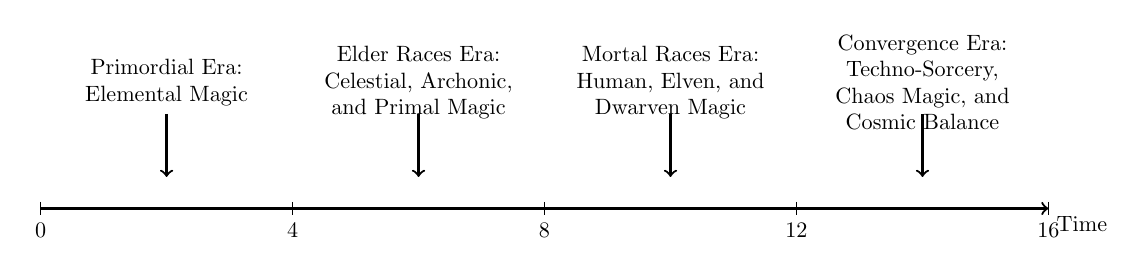
\begin{tikzpicture}[scale=0.8, transform shape]
        \draw[thick,->] (0,0) -- (16,0) node[anchor=north west] {Time};
        
        \foreach \x in {0,4,8,12,16}
            \draw (\x cm,3pt) -- (\x cm,-3pt) node[anchor=north] {\x};
        
        \node[align=center] at (2,2) {Primordial Era:\\Elemental Magic};
        \draw[thick,->] (2,1.5) -- (2,0.5);
        
        \node[align=center] at (6,2) {Elder Races Era:\\Celestial, Archonic,\\and Primal Magic};
        \draw[thick,->] (6,1.5) -- (6,0.5);
        
        \node[align=center] at (10,2) {Mortal Races Era:\\Human, Elven, and\\Dwarven Magic};
        \draw[thick,->] (10,1.5) -- (10,0.5);
        
        \node[align=center] at (14,2) {Convergence Era:\\Techno-Sorcery,\\Chaos Magic, and\\Cosmic Balance};
        \draw[thick,->] (14,1.5) -- (14,0.5);
    \end{tikzpicture}
    \caption{A timeline of major eras and paradigm shifts in the magical history of the Soluna-Gaia universe.}
    \label{fig:magic_history_timeline}
\end{figure}

The earliest known practitioners of magic in the SGU were the primordial elementals, vast and ancient beings of pure elemental energy that emerged in the chaotic formative eras of the universe. These elementals were not sapient in the conventional sense, but rather embodiments of the fundamental forces and principles that governed the cosmos, the living manifestations of the Prime Elements themselves.

According to the most ancient and esoteric of magical texts, the elementals were the first to discover the art of spellcasting, shaping the raw energies of the universe into patterns and forms that could alter the fabric of reality itself. The spells of the elementals were vast and primal, capable of creating and destroying entire worlds, of shaping the very laws of physics and magic to their will.

For eons, the elementals reigned supreme over the SGU, shaping the cosmos according to their whims and desires. But as the universe cooled and stabilized, new forms of life began to emerge, beings of matter and energy that were capable of harnessing the power of magic in their own right. The first of these were the elder races, ancient and powerful civilizations that rose to prominence in the early eras of the universe, such as the Celestials, the Archons, and the Primals.

The elder races were quick to learn the secrets of magic from the elementals, adapting and refining the primal spellcasting techniques into more sophisticated and specialized forms. The Celestials, for example, focused on the manipulation of cosmic energies and the harnessing of the power of the stars, while the Archons delved into the secrets of the mind and the manipulation of reality through thought and belief.

As the elder races spread throughout the SGU, they brought their magical knowledge and techniques with them, seeding the universe with countless magical traditions and schools of thought. From the star-forged runic magic of the Celestials to the dream-weaving sorcery of the Archons, the magic of the elder races was as diverse and wondrous as the beings themselves.

However, the reign of the elder races was not to last forever. As the eons passed, new and younger races began to emerge, beings of flesh and blood that were born of the very stuff of the universe itself. These mortal races, such as the humans, elves, and dwarves, were initially seen as primitive and unsophisticated by the elder races, lacking the vast cosmic power and knowledge that had been the birthright of their predecessors.

But the mortal races soon proved to be far more adaptable and resilient than the elder races had ever imagined. Driven by their insatiable curiosity and their need to survive and thrive in an often hostile universe, the mortal races began to learn the secrets of magic for themselves, often through a combination of trial and error, experimentation and observation, and the guidance of ancient and powerful magical mentors.

Over time, the mortal races developed their own unique magical traditions and paradigms, shaped by their own cultures, beliefs, and ways of being in the world. The human mages of the Arcanum, for example, focused on the scientific study and codification of magical principles, seeking to understand the underlying laws and mechanisms that governed the universe. The elven mystics of the Sylvastri, on the other hand, embraced a more intuitive and holistic approach to magic, seeking to attune themselves to the natural rhythms and energies of the world around them.

\begin{figure}[htb]
    \centering
    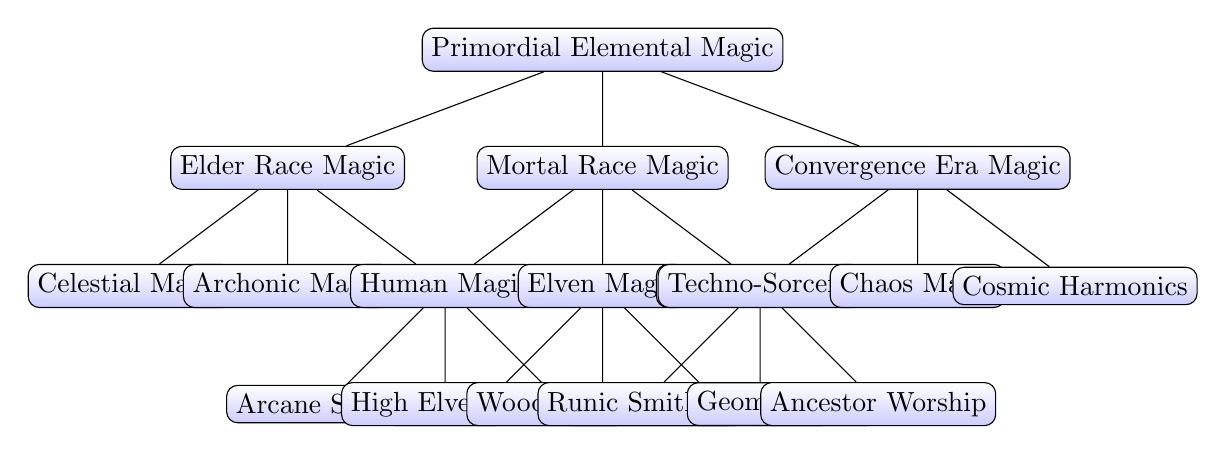
\begin{tikzpicture}[
        level 1/.style={sibling distance=40mm},
        level 2/.style={sibling distance=20mm},
        level 3/.style={sibling distance=15mm},
        every node/.style = {shape=rectangle, rounded corners, draw, align=center, top color=white, bottom color=blue!20}
    ]
        \node {Primordial Elemental Magic}
            child { node {Elder Race Magic}
                child { node {Celestial Magic}}
                child { node {Archonic Magic}}
                child { node {Primal Magic}}
            }
            child { node {Mortal Race Magic}
                child { node {Human Magic}
                    child { node {Arcane Science}}
                    child { node {Theurgy}}
                    child { node {Witchcraft}}
                }
                child { node {Elven Magic}
                    child { node {High Elven Mysticism}}
                    child { node {Wood Elven Druidry}}
                    child { node {Dark Elven Necromancy}}
                }
                child { node {Dwarven Magic}
                    child { node {Runic Smithing}}
                    child { node {Geomancy}}
                    child { node {Ancestor Worship}}
                }
            }
            child { node {Convergence Era Magic}
                child { node {Techno-Sorcery}}
                child { node {Chaos Magic}}
                child { node {Cosmic Harmonics}}
            };
    \end{tikzpicture}
    \caption{A tree diagram illustrating the evolution and development of different magical schools and disciplines over time.}
    \label{fig:magic_schools_tree}
\end{figure}

As the mortal races spread throughout the SGU, they brought their own unique perspectives and approaches to magic with them, enriching and diversifying the magical landscape of the universe. And as they encountered the elder races and the remnants of the primordial elementals, they began to learn and incorporate the ancient and primal forms of magic into their own practices, creating new and powerful hybrid traditions that blended the old and the new in fascinating and unpredictable ways.

One of the most significant events in the magical history of the SGU was the Convergence, a rare and powerful celestial alignment that occurred roughly ten thousand years ago. During the Convergence, the barriers between the dimensions and planes of reality grew thin and porous, allowing for an unprecedented exchange of magical knowledge and energy between the various races and realms of the universe.

The Convergence was a time of great upheaval and transformation, as ancient and long-forgotten forms of magic were rediscovered and new and incredible magical techniques were developed and shared. Mages from across the universe gathered in great conclaves and symposiums, sharing their knowledge and debating the fundamental nature of magic and reality itself.

It was during the Convergence that some of the greatest magical achievements and breakthroughs of the SGU were accomplished, such as the creation of the first true artificial intelligences, the development of interdimensional travel and communication, and the unlocking of the secrets of immortality and godhood. And it was also during the Convergence that some of the darkest and most terrible forms of magic were unleashed upon the universe, as rogue mages and malevolent entities sought to harness the power of the alignment for their own twisted ends.

In the aftermath of the Convergence, the magical landscape of the SGU was forever changed. New schools of magic and magical paradigms emerged, such as the techno-sorcery of the Arcanum, which sought to blend magic and technology into a seamless whole, and the chaos magic of the Entropists, which embraced the power of randomness and uncertainty as a fundamental aspect of reality.

At the same time, the Convergence also led to a greater awareness of the dangers and responsibilities of magic, as the devastating consequences of unchecked magical experimentation and hubris became all too apparent. In response, many magical societies and institutions developed strict codes of ethics and conduct for the use of magic, seeking to ensure that the power of the arcane was used responsibly and for the greater good of all.

One of the most influential of these magical institutions was the Order of the Cosmic Balance, a pan-dimensional organization of mages and scholars dedicated to maintaining the delicate equilibrium between the forces of magic and the natural laws of the universe. The Order believed that magic was a tool to be used in service of life and creation, not a weapon to be wielded for destruction and domination, and they worked tirelessly to promote this philosophy throughout the SGU.

However, not all mages and magical societies were so benevolent or altruistic in their intentions. There were many who saw magic as a means to power and control, who believed that the strong had the right to dominate and exploit the weak, and who sought to bend the very fabric of reality to their will. These dark mages and malevolent entities posed a constant threat to the stability and harmony of the SGU, and it fell to the Order and other like-minded magical defenders to stand against them and protect the innocent.

\begin{figure}[htb]
    \centering
    \begin{tikzpicture}[
        node distance=2cm,
        every node/.style={fill=white, font=\sffamily},
        every edge/.style={draw=black, very thick},
        faction/.style={rectangle, rounded corners, draw=black, very thick, minimum size=1cm, text width=2.5cm, align=center},
        influence/.style={->, >=stealth', shorten >=1pt, thick}
    ]

        % Nodes
        \node[faction] (arcanum) {Arcanum};
        \node[faction] (order) [right=of arcanum] {Order of Cosmic Balance};
        \node[faction] (technosorcery) [above=of order] {Technosorcery Guild};
        \node[faction] (chaos) [below=of order] {Chaos Mages};
        \node[faction] (sylvastri) [left=of arcanum] {Sylvastri Mystics};
        \node[faction] (entropists) [below=of chaos] {Entropists};
        
        % Edges
        \path (arcanum) edge[influence, bend left] node[align=center] {Collaborative\\Research} (technosorcery)
              (arcanum) edge[influence] node[align=center] {Knowledge\\Exchange} (order)
              (arcanum) edge[influence] node[align=center] {Philosophical\\Debates} (sylvastri)
              (order) edge[influence, bend right] node[align=center] {Ethical\\Oversight} (technosorcery)
              (order) edge[influence] node[align=center] {Conflict\\Resolution} (chaos)
              (order) edge[influence] node[align=center] {Ideological\\Opposition} (entropists)
              (chaos) edge[influence] node[align=center] {Uneasy\\Alliances} (entropists);
    \end{tikzpicture}
    \caption{A network diagram illustrating the relationships and interactions between different magical societies, institutions, and factions throughout history.}
    \label{fig:magic_factions_network}
\end{figure}

Throughout the long and tumultuous history of magic in the SGU, there have been many other significant events and paradigm shifts that have shaped the course of magical evolution and development. From the rise and fall of great magical empires to the discovery of new and incredible forms of magic, from the wars between rival magical factions to the collaborations and alliances between unlikely magical allies, the history of magic is a rich and endlessly fascinating tapestry of wonder, terror, and possibility.

And through it all, the fundamental questions and mysteries of magic have endured, the eternal enigmas that have driven the imaginations and ambitions of mages and scholars across the eons. What is the true nature of magic, and how does it relate to the fundamental structure of reality itself? What are the limits and potential of magical power, and how can it be harnessed and wielded for the betterment of all? And what does the future hold for the magical arts and sciences, as the universe continues to evolve and change in ways both wondrous and terrifying?

These are the questions that have shaped the magical history of the Soluna-Gaia universe, and they will continue to drive the ongoing story of magic and its place in the cosmos for eons to come. For as long as there are those who seek to unlock the secrets of the arcane and explore the infinite possibilities of the magical arts, the history of magic will never truly be finished, but will remain an endlessly unfolding tale of discovery, wonder, and the eternal quest for knowledge and understanding.


% Regarding the diagrams, I agree that Mermaid could be an excellent tool for visualizing some of the key concepts and relationships discussed in the paper. Some potential diagrams that could be created include:
% 
% 1. A Venn diagram showing the overlapping domains and properties of the three Prime Elements (Sun, Moon, Earth).
% 2. A flow chart illustrating the process of spellcasting, from the initial attunement to the release of magical energy.
% 3. A timeline of major events and paradigm shifts in the magical history of the SGU, such as the Convergence and the rise of different magical traditions.
% 4. A tree diagram depicting the evolution and development of different magical schools and disciplines over time.
% 5. A network diagram showing the relationships and interactions between different magical societies, institutions, and factions throughout history.
% section 5 paste end

% conclusion paste begin
\section{Conclusion and Future Directions}

In this paper, we have explored the fundamental principles and workings of magic in the Soluna-Gaia universe, from the metaphysical underpinnings of the Prime Elements to the complex celestial dynamics that shape the ebb and flow of magical energies throughout the cosmos. We have seen how magic is not merely a tool or a technology, but a profound and intrinsic aspect of the very fabric of reality, woven into the structure of space, time, and consciousness itself.

Through our examination of the history and evolution of magical traditions and paradigms in the SGU, we have traced the development of magic from its primal origins in the elemental forces of the universe to its most sophisticated and esoteric manifestations in the hands of mortal and immortal practitioners alike. We have seen how magic has shaped the course of civilizations and the destiny of entire worlds, and how it continues to be a vital and dynamic force in the ongoing story of the cosmos.

Yet for all that we have learned and discovered about magic through our research and analysis, we must also acknowledge that there is still so much that remains unknown and unexplored. The mysteries of magic are as vast and deep as the universe itself, and there will always be new frontiers to explore, new questions to ask, and new wonders to uncover.

One of the most pressing and exciting areas for future research in the field of magic is the study of cross-elemental synergies and interactions. While we have a solid understanding of the basic properties and manifestations of the individual Prime Elements, we are only just beginning to scratch the surface of how these elements can be combined and blended in novel and powerful ways. The development of new hybrid magical disciplines and techniques that draw upon multiple elemental energies could open up entirely new vistas of magical potential and possibility.

Another key area for further investigation is the relationship between magic and technology in the SGU. As we have seen throughout history, the boundaries between these two domains have always been fluid and porous, with mages and inventors alike seeking to harness the power of both in their quest for knowledge and mastery. In recent years, the rise of techno-sorcery and other hybrid magical-technological practices has only accelerated this trend, blurring the lines between the arcane and the scientific in fascinating and sometimes unsettling ways. Further research into the implications and potential of this ongoing convergence could help us to better understand and navigate the changing landscape of magic and technology in the SGU.

A third area of inquiry that holds great promise for the future of magical studies is the exploration of the psychological and cognitive dimensions of spellcasting and magical practice. While much of our understanding of magic has focused on the external manifestations and effects of spells and rituals, there is still much to be learned about the internal processes and experiences of mages themselves. By delving deeper into the mental and emotional aspects of magic, we may gain new insights into the nature of consciousness, creativity, and the human (and non-human) potential for transcendence and transformation.

Beyond these specific areas of research, there are countless other questions and enigmas that beckon to be explored in the realm of magic. From the search for the ultimate origins and destiny of magic in the universe, to the investigation of the ethical and moral dimensions of magical practice, to the study of the role of magic in shaping the evolution and ecology of life in the cosmos, the possibilities for further inquiry are truly endless.

As we look to the future of magical studies in the SGU, it is clear that we stand at the threshold of a new era of discovery and revelation. With each passing day, new magical phenomena are being documented, new theories and paradigms are being proposed, and new generations of mages and scholars are taking up the mantle of exploration and investigation.

It is our hope that this paper has provided a solid foundation and framework for understanding the fundamentals of magic in the SGU, and that it will serve as a springboard for further research and inquiry in the years and decades to come. We believe that the study of magic is not only a fascinating and rewarding intellectual pursuit in its own right, but also a vital and necessary endeavor for anyone who seeks to comprehend the true nature and potential of the universe we inhabit.

For magic is not simply a tool or a technology, but a mirror that reflects the deepest truths and mysteries of existence itself. By gazing into that mirror with open minds and hearts, we may catch a glimpse of the infinite wonders and possibilities that lie within and beyond the boundaries of our current understanding. And in doing so, we may take another step forward on the great and eternal journey of discovery and enlightenment that is the birthright and destiny of all living beings in the cosmos.

It is in this spirit of wonder, curiosity, and reverence that we conclude our exploration of the magical arts and sciences in the Soluna-Gaia universe. May the light of knowledge and understanding guide us ever onward, and may the magic of the cosmos continue to inspire and transform us all, now and forever more.
% conclusion paste end
% \section{Conclusion}
% In conclusion, this paper has presented a model for understanding the magical cosmology of the Soluna-Gaia universe. The three Prime Elements of Sun, Moon, and Earth generate the fundamental metaphysical forces that shape the SGU and give rise to the various expressions of magic. By studying the principles and interactions of Solar, Lunar, and Terrestrial energy, we can better understand the nature of thaumaturgy and its role in the physical and historical structure of the SGU.
% 
% Our model provides a framework for categorizing magical phenomena, predicting the outcomes of spells, and interpreting the metaphysical significance of celestial events. It also offers insight into the historical development of magical traditions and institutions in the SGU, and the ways in which magic has shaped the course of civilizations.
% 
% However, many questions remain unanswered. How exactly do the Prime Elements generate magical energy? What is the nature of the link between the physical celestial bodies and their metaphysical domains? How do individual mages form attunements to the different Elements? What are the limits of magic's ability to reshape reality?
% 
% Future research could explore these questions through advanced thaumaturgical experiments, delve into the historical records of lost magical traditions, or seek insight from other planes of existence. As our understanding of magic grows, so too will our appreciation for the profound complexity and wonder of the Soluna-Gaia universe.

\bibliographystyle{plainnat}
\bibliography{references}

\end{document}
